%!TEX root = ../main.tex
\chapter{Bluetooth}\label{text}
\section{Bluetooth}

Bluetooth is a widely adopted wireless technology that has seen rapid growth over the past decade. Originally developed to eliminate the need for short-range wired connections, Bluetooth is now used in countless applications—from music and video streaming to medical devices requiring continuous data updates. 
While it operates similarly to WiFi in some respects, the key difference is its scope: WiFi connects multiple devices to the internet, whereas Bluetooth focuses on direct device-to-device communication and offers more diverse use cases \cite{intelBLEguide}.

Another distinction is how Bluetooth is optimized for low-latency applications that transmit small bursts of data quickly and efficiently.
 This makes it ideal for scenarios where power conservation and responsiveness are more important than high throughput.

\subsection{Bluetooth Types}

There are two main types of Bluetooth technology: \textit{Bluetooth Basic Rate (BR)}, also referred to as \textit{Bluetooth Classic}, and \textit{Bluetooth Low Energy (BLE)}. Of the two, BLE has gained far more traction in modern applications.

Bluetooth Basic Rate is the older of the two technologies, supported in versions 1.0 through 3.0. It is primarily used for wireless audio streaming in devices like headphones, speakers, and in-car entertainment systems, and it relies on point-to-point communication.

Bluetooth Low Energy, introduced in version 4.0 and further enhanced in version 5.0, offers a broader range of capabilities. In addition to supporting audio and data transfer, BLE enables device networking and location services. It supports multiple communication topologies including point-to-point, mesh, and broadcast, making it far more versatile than its predecessor. One of BLE’s standout features is its utility in high-accuracy location services. By leveraging nearby devices, BLE can determine relative positioning and provide precise location tracking.

\section{Pairing-Based Network}

The core of Bluetooth is creating a network where two (or slightly more) devices pair with each other, since Bluetooth was designed to replace corded connections. The devices being paired can be broken down into the \textit{Central} and \textit{Peripheral(s)}. These terms are specific to newer Bluetooth standards and can be used interchangeably with the older terms \textit{Master} and \textit{Slave}.

The Central device coordinates the data being sent between it and any Slaves. This includes handling time synchronization, sleep scheduling, and configuring the channels used through frequency hopping \cite{nextgenBLE}. Peripheral devices can communicate bi-directionally with the Master device, sending or receiving data depending on the request.

Figure \ref{fig:centralperipheral} shows an example of Central and Peripheral devices. Classic Bluetooth includes two network topology configurations: \textbf{Piconet} and \textbf{Scatternet}.

\begin{figure}[h]
    \caption{Central and Peripheral device relationship}
    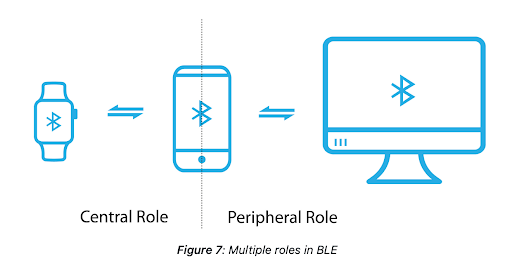
\includegraphics[scale=.7]{centralperipheral.png}
    \label{fig:centralperipheral}
    \end{figure}

\subsection{Piconet}

A piconet is a type of ad hoc network topology that operates without preestablished infrastructure. Devices in a piconet communicate directly with one another without the need for a centralized device like a router or access point. The network is organized with one central device and one or more peripheral devices. A single central can support up to seven active peripherals, while each peripheral can only connect to one central \cite{nextgenBLE}. The central manages the timing and synchronization of all devices in the piconet. Peripheral devices cannot communicate directly with each other; the central acts as a relay, forwarding data between them.

Figure \ref{fig:piconet} shows the structure of a piconet.

\begin{figure}[h]
    \caption{Piconet Topology}
    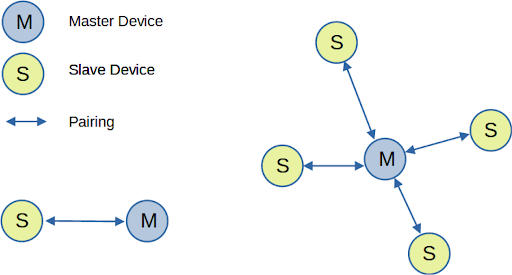
\includegraphics[scale=.7]{piconet.png}
    \label{fig:piconet}
    \end{figure}

All connections made using a BR/EDR controller occur within a piconet. BR/EDR devices communicate over the same physical channel by synchronizing with a shared clock and hopping sequence \cite{bluetoothcorespec6}. The piconet clock follows the central device's clock configuration, and the hopping sequence is also derived from the central’s clock and Bluetooth device address.

Multiple independent piconets can exist in the same area. Each operates on a separate channel and is organized around a different central device. Bluetooth devices can also participate in multiple piconets simultaneously. While a Bluetooth device can only act as the central in one piconet at a time, it can serve as a peripheral in several.


\subsection{Scatternet}

A scatternet is formed by connecting multiple piconets together. Unlike a piconet, a peripheral in a scatternet can connect to multiple central devices. Central devices can also connect to each other, sometimes serving dual roles as both central and peripheral.

For example, a scatternet might include a central laptop connected to a Bluetooth speaker, while also acting as a peripheral to a smartphone and printer. Figure \ref{fig:scatternet} shows a diagram of a typical scatternet. Despite the increased complexity, peripherals still do not communicate directly with each other.

Piconets and scatternets are associated with Classic Bluetooth but are still supported in BLE and later Bluetooth versions \cite{nextgenBLE}. Although BLE—with its advertising mode—has seen growing popularity, traditional Bluetooth methods still offer advantages such as added security during pairing. BLE services enhance the piconet and scatternet model, providing better security, more efficient pairing, and broader support for services.

\begin{figure}[h]
    \caption{Scatteret Topology}
    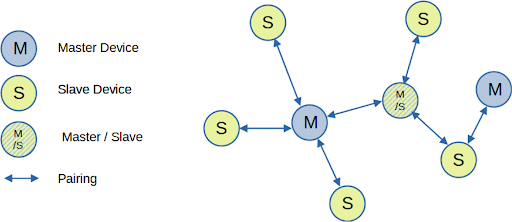
\includegraphics[scale=.7]{scatternet.png}
    \label{fig:scatternet}
    \end{figure}

\section{BLE Mesh Networks}

Mesh networking, introduced with BLE, marks a significant evolution in Bluetooth topologies. In a mesh network, nodes are arranged in a self-configuring mesh, where each node relays traffic between peers when the destination is not directly connected \cite{buildingBLEsystems}.

This structure ensures a reliable path for data packets. If one path is blocked or unavailable, the network reroutes traffic dynamically. The self-organizing nature of mesh networks means they adapt in real-time to changes, such as nodes joining, leaving, or moving within the network.

For example, Figure \ref{fig:mesh} shows Device 1 out of range of Device 3. Device 2, within range of both, acts as a router forwarding messages between them.
\begin{figure}[h]
    \caption{Mesh topology}
    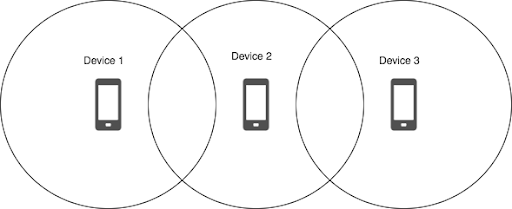
\includegraphics{mesh.png}
    \label{fig:mesh}
    \end{figure}

\section{Broadcast Network from LE}

BLE introduces a new feature called \textit{advertising mode}, which operates differently from the traditional pairing between a central and peripheral. In advertising mode, a device broadcasts data openly to any BLE devices within range that are tuned to the same channel. These listening devices can receive the data and use it as needed—without any pairing, connection, or formal association.

This topology loosely resembles a multi-peripheral piconet, but with a key difference: advertising mode removes the need for a dedicated central or established links. There’s no synchronization or connection—just open broadcasting.

Advertising mode has been a major factor in expanding the possibilities of Bluetooth. By offloading the overhead of pairing, BLE made room for a wider variety of lightweight, low-latency applications. This performance shift is part of why so many modern devices—from smart beacons to virtual reality headsets—are feasible today. Devices like VR headsets, which require fast, efficient data sharing without constant handshaking, would be nearly impossible to build the same way without Bluetooth.

\section{Connections and Mixed Topology}

A connection becomes necessary when data needs to flow in both directions or when there’s more data than can fit into the two available advertising payloads. Connections in BLE are more persistent—they allow devices to remember each other and avoid reestablishing the connection every time. Once established, connections support periodic data exchanges between two devices.

This connection-based pairing is what underpins piconets and scatternets. These connections are private by design: only the two participating devices exchange data (barring external sniffing). As covered earlier, connections involve one central device and one or more peripheral devices.

BLE networks can also incorporate mixed topology configurations depending on the use case. A device that supports both BR/EDR and LE can serve as a bridge between traditional Bluetooth and BLE communication, enabling broader interoperability across protocols. The possibilities for combining these configurations are only constrained by the capabilities of the individual devices' radios and protocol stacks.

Figure \ref{fig:mixedtopology} provides an example of a mixed topology Bluetooth network.

\begin{figure}[h]
    \caption{Mixed Topology}
    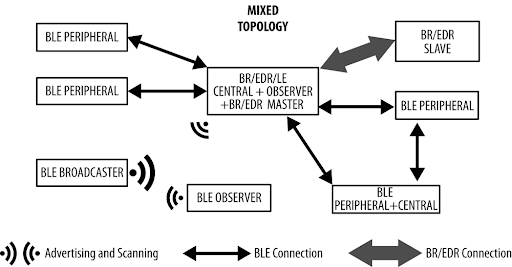
\includegraphics{mixedtopology.png}
    \label{fig:mixedtopology}
    \end{figure}

\section{SCO and ACL Logical Transports}

\subsection{BR/EDR Asynchronous Connection-Oriented (ACL)}

ACL links are the primary way Bluetooth devices using BR/EDR exchange general data. These links handle both control signals (like LMP and L2CAP) and typical user data. ACL is \textit{asynchronous}, meaning data is sent when available rather than on a fixed schedule.

Every Peripheral in a Bluetooth piconet gets one default ACL link to the Central. This link is established when the device first connects and is identified by a Logical Transport Address (LT\_ADDR) assigned by the Central. This LT\_ADDR is also used when identifying the physical connection between devices.

However, because multiple types of logical transports (like SCO links, which are used for voice) might use the same LT\_ADDR, it’s not enough to identify the ACL connection by LT\_ADDR alone. Devices also rely on the packet type to tell them which kind of transport is being used.

ACL links can also carry isochronous data—data that needs to arrive on time, like audio streams—by setting them to automatically drop old packets. At the same time, asynchronous traffic (like file transfers) can still be sent if it’s marked not to auto-flush. This means both types of traffic can share the same ACL link if configured correctly.

If the ACL link is removed or if the device loses sync with the piconet, all other connections between the Central and that Peripheral (like SCO) are also dropped immediately \cite{bluetoothcorespec6}.

\subsection{BR/EDR Synchronous Connection-Oriented (SCO)}

SCO links are designed specifically for real-time data like voice. They create a fixed, circuit-like connection between a Central and a Peripheral by reserving slots on the Bluetooth physical channel. These connections carry 64 kbps of data, usually for audio, and are synchronized with the piconet’s clock.

There are several SCO configurations that balance audio quality, latency, and bandwidth usage. Every SCO connection uses the same LT\_ADDR as the ACL link, so to identify an SCO packet, a device must look at the slot number, packet type, and LT\_ADDR together.

Even though SCO reserves bandwidth, the system can override these slots if higher-priority data (like control messages over ACL) needs to get through. This helps maintain overall system reliability and meet Quality of Service (QoS) requirements.

Unlike ACL links, SCO links don’t carry complex protocols or layered data structures. They just send a steady stream of audio—either in a standard format or as raw data for the application to decode \cite{bluetoothcorespec6}.

\section{Bluetooth Low Energy Broadcasting and Observing}

Bluetooth Low Energy devices communicate with the outside world in two primary ways: \textit{broadcasting} and \textit{connecting}. Both methods are governed by the Generic Access Profile (GAP), which outlines how devices discover and interact with each other \cite{gettingstartedwble}.

Broadcasting enables BLE devices to send data one-way to any scanner or receiver within range. It’s a form of open communication where any nearby device capable of listening can receive the broadcasted data. Figure \ref{fig:broadcastobserve} illustrates this communication model. In the diagram, two roles are shown: the \textit{Broadcaster}, which periodically sends non-connectable advertising packets, and the \textit{Observer}, which continually scans for those packets \cite{gettingstartedwble}.

\begin{figure}[h]
    \caption{Broadcasting and Observing}
    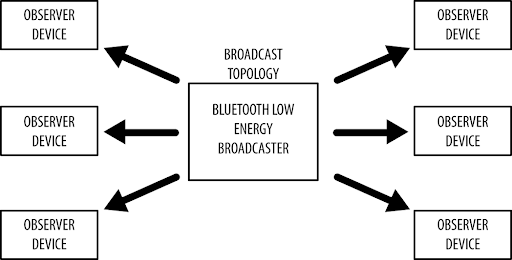
\includegraphics{broadcastobserve.png}
    \label{fig:broadcastobserve}
    \end{figure}

Broadcasting is a key concept in BLE because it’s the only mechanism that allows a device to communicate with multiple other devices simultaneously. This functionality is made possible by BLE’s advertising feature.

A standard advertising packet contains a 31-byte payload, which includes information about the broadcasting device and what it offers. This data can be customized to suit different applications, providing useful context to observing devices. If 31 bytes isn’t enough, BLE allows for a secondary packet called a \textit{Scan Response}, which provides an additional 31 bytes of payload. Observers can request this secondary data if they need more information \cite{gettingstartedwble}.

Broadcasting is quick, efficient, and ideal for sending small amounts of data on a regular schedule to multiple receivers. However, it does come with limitations—particularly around security. Since any device within range can intercept a broadcast, there’s virtually no privacy. Because of this, broadcasting isn’t well-suited for transmitting sensitive or private data.
\section{Bluetooth Protocols and Profiles}

Bluetooth has always had a distinction between protocols and profiles. A protocol is a lower layer foundational block that gets used by all devices that have Bluetooth capabilities. They deal with the layers that implement the different packet formats, routing, encoding, decoding, and multiplexing that allows data to be properly sent between peers \cite{gettingstartedwble}. Profiles are ``vertical slices'' of functionality that encompass either fundamental modes of operation common to all devices (such as the Generic Access Profile and Generic Attribute Profile) or support specific use cases (like the Proximity Profile or Glucose Profile). They essentially define how protocols should be applied to accomplish a particular objective, whether general or specialized.

\section{Bluetooth Low Energy Profiles}

Profiles specify how BLE protocols are to be used to achieve interoperability and support a wide range of applications. These profiles fall into two primary categories: generic profiles, which are fundamental to all BLE operations, and use-case-specific profiles, which are built on top of the generic layers to support particular functionalities.

\subsection{Generic Profiles}

Generic profiles are defined by the Bluetooth Core Specification and provide the foundational mechanisms required for BLE communication. These profiles ensure that devices from different manufacturers can interoperate seamlessly. Two such profiles—Generic Access Profile (GAP) and Generic Attribute Profile (GATT)—are mandatory for all BLE-compliant devices and serve as the cornerstones of BLE communication.

\subsubsection{Generic Access Profile (GAP)}

The Generic Access Profile defines the roles, procedures, and operational modes required for device discovery, broadcasting, connection establishment, connection management, and security negotiation. GAP operates as the top-level control layer within the BLE protocol stack, orchestrating the basic behaviors necessary for device interaction. All BLE devices must implement and conform to the GAP specifications to ensure compatibility and reliable communication.

\subsubsection{Generic Attribute Profile (GATT)}

GATT focuses primarily on how data is exchanged. GATT defines a universal data model and a set of procedures that enable devices to discover, read, write, and notify data values. It functions as the uppermost data layer in BLE and serves as the foundational framework upon which most BLE applications and services are constructed.

Due to their foundational roles, GAP and GATT are commonly exposed through application programming interfaces (APIs), making them the primary entry points for developers interacting with the BLE protocol stack.

\subsection{Use-Case-Specific Profiles}

Beyond the generic profiles, the Bluetooth Special Interest Group (SIG) has defined a series of use-case-specific profiles. These profiles are designed to standardize behavior for specific applications and are exclusively built upon the GATT framework. At the time of writing, no BLE profiles exist outside the GATT structure. However, the introduction of connection-oriented L2CAP channels in Bluetooth version 4.1 may pave the way for future GATT-less profiles.

\subsubsection{SIG-Defined GATT-Based Profiles}

The Bluetooth SIG provides an extensive catalog of standardized profiles, each tailored to support a specific application or device type. These profiles fully specify the required procedures and data formats, facilitating rapid development and ensuring interoperability across implementations.

Examples of SIG-defined GATT-based profiles include:

\begin{itemize}
    \item \textbf{Find Me Profile:} Enables physical location of nearby BLE devices (e.g., locating a lost phone or keyring).
    \item \textbf{Proximity Profile:} Detects when a connected device moves beyond a designated range, triggering alerts.
    \item \textbf{HID over GATT Profile:} Facilitates the transmission of Human Interface Device (HID) data over BLE for peripherals such as keyboards, mice, and remote controls.
    \item \textbf{Glucose Profile:} Securely transmits glucose measurement data for health monitoring applications.
    \item \textbf{Health Thermometer Profile:} Enables transfer of body temperature readings from wearable or medical devices.
    \item \textbf{Cycling Speed and Cadence Profile:} Allows cycling sensors to relay speed and cadence information to companion applications or devices.
\end{itemize}

A comprehensive list of SIG-adopted profiles is available on the Bluetooth SIG Specification Adopted Documents webpage. Developers may also consult the Bluetooth Developer Portal for up-to-date listings of adopted services and characteristics.

\subsubsection{Vendor-Specific Profiles}

While the SIG provides a broad range of standardized profiles, the BLE specification also permits the definition of vendor-specific profiles. These profiles are often developed to support proprietary use cases not covered by SIG standards. Vendor-specific profiles can be implemented privately between two devices (such as with a health accessory and a smartphone) or published to enable broader adoption.

Notable examples of vendor-defined profiles include:

\begin{itemize}
    \item \textbf{Apple iBeacon:} A proprietary proximity-sensing profile used for indoor positioning and location-based services.
    \item \textbf{Apple Notification Center Service (ANCS):} Enables wearable devices or external displays to access and display iOS notifications.
\end{itemize}

These profiles demonstrate the flexibility of the BLE specification in accommodating both standardized and proprietary communication models.

\section{Bluetooth Low Energy (BLE) Architecture}

Although most users will only ever interact with the top layers of the Bluetooth Low Energy (BLE) protocol stack, having a basic understanding of the full stack can provide helpful context. This overview lays the groundwork for understanding how BLE devices work and why each part of the system is important. A typical single-mode BLE device is made up of three main parts: the controller, the host, and the application. Each of these parts contains multiple layers, each responsible for specific tasks that allow the device to communicate and perform its intended functions. Figure \ref{fig:bleprotocolstack} shows the BLE protocol stack.

\begin{figure}[h]
    \caption{BLE Protocol Stack}
    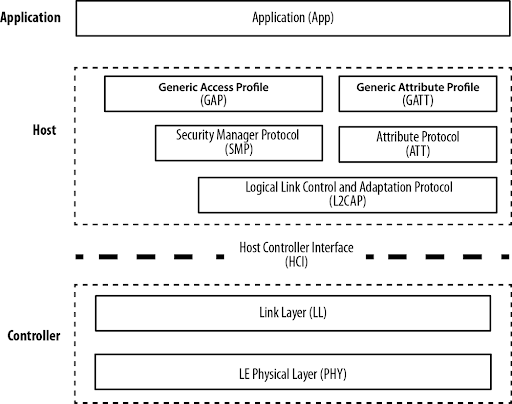
\includegraphics[scale=.7]{bleprotocolstack.png}
    \label{fig:bleprotocolstack}
    \end{figure}

\subsection{Application}

The application layer sits at the top of the BLE protocol stack. It includes all the logic, data handling, and user interface components that define how a device behaves in a specific use case. This layer is highly customized and varies from one implementation to another \cite{nextgenBLE}.

\subsection{Host}

Below the application is the host, which includes several critical layers that manage communication and device behavior:

\begin{itemize}
    \item \textbf{Generic Access Profile (GAP):} Controls how devices advertise themselves, discover others, establish connections, and manage roles and security \cite{nextgenBLE}.
    \item \textbf{Generic Attribute Profile (GATT):} Organizes and manages how data is exchanged between connected devices.
    \item \textbf{Logical Link Control and Adaptation Protocol (L2CAP):} Handles multiplexing and segmentation of data packets.
    \item \textbf{Attribute Protocol (ATT):} Supports data operations such as reads and writes via attribute handles.
    \item \textbf{Security Manager (SM):} Manages pairing, authentication, and encryption.
    \item \textbf{Host Controller Interface (HCI) – Host Side:} Facilitates communication between the host and controller \cite{nextgenBLE}.
\end{itemize}

\subsection{Controller}

At the bottom of the Bluetooth stack, the controller is responsible for radio operations and low-level data transport. It typically includes the following components:

\begin{itemize}
    \item \textbf{Physical Layer (PHY):} Manages the actual transmission and reception of radio signals.
    \item \textbf{Link Layer (LL):} Controls advertising, scanning, and maintaining connections.
    \item \textbf{HCI (Controller Side):} Complements the host side of HCI to enable structured data flow between layers \cite{nextgenBLE}.
\end{itemize}

According to the Bluetooth Core Specification, a Bluetooth implementation includes a single controller, which may be configured as one of the following:

\begin{itemize}
    \item A \textbf{BR/EDR controller}, containing the Radio, Baseband, Link Manager, and optionally HCI.
    \item An \textbf{LE controller}, including the LE PHY, Link Layer, and optionally HCI.
    \item A \textbf{dual-mode controller} that combines both BR/EDR and LE controller functions into a single unit.
\end{itemize}

Together, these layers ensure that BLE devices can connect reliably and communicate efficiently. This layered architecture is often described from the bottom up — starting at the antenna and PHY layer and moving up through the stack to the user-facing application.

\section{BLE Link Layer and Device Addressing}

In the Bluetooth Low Energy (BLE) protocol stack, the Link Layer serves as a crucial interface between the Physical Layer—which handles the actual radio transmission—and the upper protocol layers. It acts as the controller for radio operations and is essential for managing the states and timing mechanisms that define BLE communication. One of the key responsibilities of the Link Layer is to abstract the radio hardware, allowing higher-level layers to interact with it through the Host Controller Interface (HCI) \cite{introtoble}. 

In addition to timing and control, the Link Layer manages several hardware-accelerated tasks. These include generating cyclic redundancy checks (CRC) for error detection, producing random numbers for cryptographic operations, and performing encryption to secure data transfer \cite{introtoble}. These operations ensure the performance, integrity, and security of BLE communications.

\subsection{Link Layer States}

BLE devices operate in a well-defined set of five main states, each with specific behaviors and transitions:

\begin{itemize}
    \item \textbf{Standby:} This is the default state, where the radio is idle and not transmitting or receiving any packets.
    \item \textbf{Advertising:} In this state, the device broadcasts data packets at regular intervals, making itself discoverable to other devices.
    \item \textbf{Scanning:} Devices in this state listen for advertising packets from others, searching for devices they might want to connect with.
    \item \textbf{Initiating:} When a scanning device decides to connect to an advertising device, it enters this state and sends a connection request.
    \item \textbf{Connected:} A persistent communication link is established. Devices in this state can exchange data regularly. The device that initiated the connection becomes the master, while the other becomes the slave \cite{introtoble}.
\end{itemize}

This framework enables BLE to support dynamic and responsive device discovery and communication, while keeping energy consumption minimal.
\section{Advertising, Scanning, and Connecting}

Advertising and scanning are complementary operations: advertising devices periodically transmit small packets of data, while scanning devices listen for and interpret these packets. If the advertiser allows connections, and a scanning device decides to initiate one, both devices transition into the connected state \cite{introtoble}. These processes form the backbone of BLE interactions and are covered in more depth in subsequent chapters of most BLE technical literature.

\section{Bluetooth Device Address}

Every Bluetooth device is identified by a 48-bit device address, which serves a function similar to a MAC address in networking. BLE supports two major types of device addresses: public addresses and random addresses, which influence how discoverable and trackable a device is.

\subsection{Public Address}

A public address is a globally unique, fixed identifier that is factory-programmed and registered with the IEEE. Because of this registration requirement, it ensures uniqueness across all BLE devices worldwide. However, it can also present privacy concerns, since it does not change and is easily traceable \cite{introtoble}.

\subsection{Random Address}

Random addresses, by contrast, provide more flexibility and are often preferred in consumer devices to protect user privacy. These addresses can either be static or private, and they do not require IEEE registration.

\begin{itemize}
    \item \textbf{Static Address:} Used as a drop-in replacement for public addresses. A static address remains the same between sessions but can be regenerated at boot or kept for the lifetime of the device until a power cycle occurs.
    \item \textbf{Private Addresses:} These are designed to change regularly and enhance privacy. They come in two subtypes:
    \begin{itemize}
        \item \textbf{Non-resolvable private addresses} are temporary, randomly generated, and cannot be traced back to a specific device. They are rarely used due to limited functionality.
        \item \textbf{Resolvable private addresses} use an Identity Resolving Key (IRK) and a random number to generate temporary addresses. These change over time, making the device hard to track by unknown parties. However, trusted or bonded devices that have the IRK stored can resolve these addresses, allowing them to re-identify the device securely \cite{introtoble}.
    \end{itemize}
\end{itemize}

This system allows BLE to balance two key goals: persistent connectivity with trusted devices and protection against unwanted tracking or eavesdropping by unknown entities.

\section{Host Controller Interface (HCI) Layer}

The Host Controller Interface (HCI) serves as the communication bridge between the host and controller layers in a Bluetooth system. These components can be implemented on the same chipset or on separate chipsets. When they are on separate chipsets, HCI is critical for enabling interoperability and communication between them. In such cases, HCI defines both the standardized protocol and the physical transport mechanisms that facilitate message exchange. As shown in Figure \ref{fig:hosthcicontroller}, the host, HCI, and controller are depicted as distinct components. HCI commonly uses transport technologies such as UART, USB, and SDIO to establish physical connections between the host and controller. When the host and controller are integrated on the same chipset, HCI functions as a logical interface rather than a physical one \cite{introtoble}.

\begin{figure}[h]
    \caption{Host, HCI, and Controller components}
    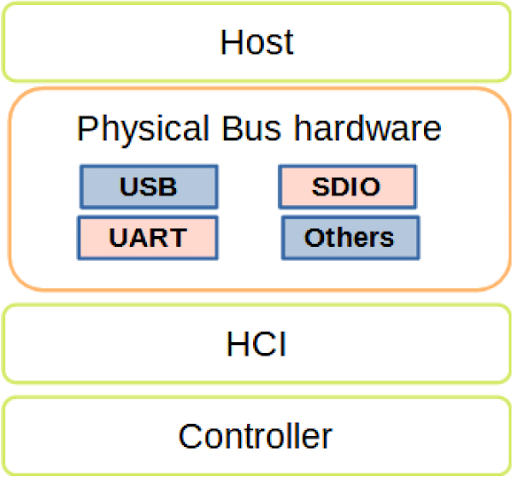
\includegraphics[scale=.6]{hosthcicontroller.png}
    \label{fig:hosthcicontroller}
    \end{figure}

\subsection{Universal Asynchronous Rx/Tx (UART)}

UART is a serial communication protocol that uses wired connections to exchange data between devices. It is commonly found in integrated circuits and is especially favored in devices like mobile phones and laptops, where the entire Bluetooth stack is implemented on a single chipset. UART is also well-suited for small, resource-constrained devices powered by microcontrollers, as it is lightweight and efficient in its use of system resources \cite{nextgenBLE}.

In the context of the HCI UART protocol, four types of packet transmissions are defined: the Command packet (identified by 0x01), Event packet (0x04), Asynchronous Connection-Less (ACL) packet (0x02), and Synchronous Connection-Oriented (SCO) packet (0x03). Because the receiving HCI layer cannot distinguish these packet types based on content alone, each transmission begins with a leading byte — known as an indicator — which acts as a header to identify the type of packet that follows \cite{nextgenBLE}.

\section{Connection}

To establish a connection in Bluetooth Low Energy (BLE), the central device begins by scanning for advertising peripheral devices that are currently accepting connection requests. Advertising packets can be filtered based on the Bluetooth Address or the contents of the advertising data itself. Once a suitable advertiser is detected, the master sends a connection request packet. If the slave responds, a connection is established \cite{gettingstartedwble}.

This connection request packet includes several critical parameters:
\begin{itemize}
    \item \textbf{Frequency hop increment:} Defines the hopping sequence used for the duration of the connection.
    \item Three additional connection parameters:
    \begin{itemize}
        \item \textbf{Connection interval:} The time between the start of two consecutive connection events. This can range from 7.5 ms (for high throughput) to 4 seconds (for minimal power usage).
        \item \textbf{Slave latency:} The number of connection events the slave is allowed to skip without causing a disconnection.
        \item \textbf{Connection supervision timeout:} The maximum allowed time between receiving valid packets before the connection is considered lost \cite{gettingstartedwble}.
    \end{itemize}
\end{itemize}

Once connected, communication happens through repeated connection events — periodic time slots where the master and slave take turns exchanging packets. A connection event:
\begin{itemize}
    \item Always begins with a packet from the central.
    \item Requires the peripheral to respond if it receives a packet.
    \item Continues until both sides have no more data to send.
    \item Is repeated at the connection interval until the connection is either closed or lost.
    \item Can be closed by either the master or the slave. If the central sends a packet and does not receive a response, it waits until the next connection event to resume \cite{introtoble}.
\end{itemize}

To manage interference and ensure privacy or security, BLE supports a white list mechanism at the Link Layer. This list defines which Bluetooth device addresses are of interest. Devices not on the list are ignored — their advertising (by scanners) or connection request packets (by advertisers) are simply dropped \cite{gettingstartedwble}.

\section{Services and Characteristics}

\subsection{Attribute Protocol (ATT)}

The Attribute Protocol (ATT) defines how a server exposes its data to a client, and how that data is organized and accessed in a Bluetooth Low Energy (BLE) system \cite{introtoble}.

\subsubsection{Roles in ATT}

There are two main roles in ATT communication:
\begin{itemize}
    \item \textbf{Server:} The server is the device that stores and exposes data, and may allow certain behaviors to be remotely controlled. It receives commands from peer devices and sends responses, notifications, or indications in return. For example, a thermometer acts as a server when it provides access to its current temperature, unit of measurement, battery level, or the interval at which it records readings. Instead of requiring the client to repeatedly poll for changes, the server can proactively notify the client when data updates occur \cite{introtoble}.
    \item \textbf{Client:} The client is the device that reads data from the server or controls the server's behavior. It sends commands and requests, and accepts incoming notifications and indications. In the thermometer example, a mobile device that connects to the thermometer and reads temperature values is operating as the client \cite{introtoble}.
\end{itemize}

\subsubsection{Data Format: Attributes}

The data exposed by the server is organized into attributes. An attribute is a general term for any piece of data available on the server, such as services or characteristics (described later).

Each attribute consists of the following elements:
\begin{itemize}
    \item \textbf{Attribute Type (UUID):} This is a Universally Unique Identifier (UUID) used to distinguish the type of data.
    \begin{itemize}
        \item A 16-bit UUID is used for Bluetooth SIG-adopted attributes.
        \item A 128-bit UUID is used for custom or vendor-specific attributes defined by developers \cite{introtoble}.
    \end{itemize}
    \item \textbf{Attribute Handle:} This is a 16-bit value that acts like an address assigned by the server to each of its attributes. The handle uniquely identifies an attribute during the lifetime of the connection, allowing the client to reference it directly. Handle values range from 0x0001 to 0xFFFF, while 0x0000 is reserved \cite{introtoble}.
    \item \textbf{Attribute Permissions:} Permissions control whether an attribute can be read, written, notified, or indicated, and what security requirements are necessary for each operation. These permissions are not specified within ATT itself, but are defined at a higher layer—typically the GATT (Generic Attribute Profile) or application layer \cite{introtoble}.
\end{itemize}
\section{Profiles}

\subsection{Generic Attribute Profile (GATT)}

The Generic Attribute Profile (GATT) defines how BLE devices organize, expose, and exchange data over a connection. It builds directly on top of the Attribute Protocol (ATT), using it as the transport layer for transmitting structured data known as attributes \cite{introtoble}.

GATT introduces a hierarchical data model centered around three key concepts:
\begin{itemize}
    \item \textbf{Services}
    \item \textbf{Characteristics}
    \item \textbf{Profiles} \cite{introtoble}
\end{itemize}

These elements allow BLE devices to encapsulate user-facing data and device functionality in a standardized, interoperable way. All BLE application-level interactions happen within the framework defined by GATT \cite{gettingstartedwble}.

\subsection{GATT Roles}

Like ATT, GATT supports client and server roles, which are dynamic per transaction rather than fixed per device. This means a single device can simultaneously act as a GATT server for one connection and a GATT client in another \cite{introtoble}.

\begin{itemize}
    \item \textbf{GATT Server:} Stores and exposes attributes to the client. It responds to requests and may send unsolicited updates via notifications or indications. Every BLE device must at least support a minimal GATT server, even if only to respond with error codes \cite{gettingstartedwble}.
    \item \textbf{GATT Client:} Initiates communication by performing service discovery, reading/writing attributes, and subscribing to updates. The client has no prior knowledge of the server’s structure—it learns through discovery procedures \cite{gettingstartedwble}.
\end{itemize}

\subsection{Services}

A service is a logical grouping of one or more attributes that collectively provide a certain function on the server. A service always includes at least one characteristic, and often contains supporting attributes like declarations, descriptors, and included services (used to reference other services) \cite{introtoble}.
\begin{itemize}
    \item \textbf{Primary Services:} Represent core functionality (e.g., Battery Service).
    \item \textbf{Secondary Services:} Offer auxiliary support and must be referenced by primary services (rarely used) \cite{introtoble}.
\end{itemize}

The Bluetooth SIG maintains a set of adopted services with published specifications to ensure interoperability across vendors. If a product claims compliance with one of these services, it must strictly follow its specification \cite{introtoble}.

\subsection{Characteristics}

A characteristic is the smallest logical unit of user-accessible data on a BLE server. It always belongs to a service and includes:
\begin{itemize}
    \item \textbf{Value:} The actual data being exposed.
    \item \textbf{Properties:} Operations permitted on the value (e.g., read, write, notify, indicate).
    \item \textbf{Descriptors:} Metadata about the value (e.g., format, units, configuration settings) \cite{introtoble}.
\end{itemize}

For example, the battery level characteristic within the Battery Service lets clients read the device's current power level \cite{introtoble}.

\subsection{Profiles}

While services and characteristics define how data is stored and exposed on the server, profiles describe how clients and servers interact, including service usage, connection procedures, and security requirements. Profiles are not discovered over BLE connections like services are; instead, they exist as specification documents, often adopted by the Bluetooth SIG. These define how multiple services should be used together to achieve specific use cases (e.g., Heart Rate Profile, Blood Pressure Profile) \cite{introtoble}.

Each profile specification includes:
\begin{itemize}
    \item Required services and characteristics
    \item Interaction behaviors for both server and client
    \item Connection and security requirements
    \item Example usage diagrams and workflows \cite{introtoble}
\end{itemize}

\section{Nordic Semiconductor}

\subsection{nRF Connect}

nRF Connect for Mobile—formerly known as the nRF Master Control Panel—is a feature-rich application designed for developers working with Bluetooth Low Energy (BLE) devices. Created by Nordic Semiconductor, this free app is available on both Android and iOS platforms and is widely regarded as one of the most powerful tools for BLE development and testing \cite{buildingBLEsystems}.

The application supports numerous Bluetooth SIG-adopted profiles, including Over-the-Air Device Firmware Updates (OTA DFU), making it especially useful for firmware deployment and debugging \cite{buildingBLEsystems}.

\subsubsection{Key Features} \cite{buildingBLEsystems}:
\begin{itemize}
    \item \textbf{BLE Device Scanning with RSSI Graphs:} Visualize signal strength (RSSI) for nearby devices in real-time.
    \item \textbf{Advertisement Data Parsing:} Inspect general advertisements and manufacturer-specific payloads.
    \item \textbf{GATT Client Functionality:} Connect to BLE peripherals and display their services and characteristics.
    \item \textbf{Characteristic Interaction:} Perform reads, writes, and observe values from server-side characteristics.
    \item \textbf{Support for Notifications and Indications:} Enable and receive updates directly from connected devices.
    \item \textbf{GATT Server Emulation:} Simulate a GATT server with built-in configuration presets.
    \item \textbf{OTA Firmware Updates:} Flash firmware over-the-air for supported devices.
    \item \textbf{Automated Testing:} Execute test cases defined in XML scripts for BLE device behavior validation.
    \item \textbf{UART Service Support:} Communicate via UART-over-BLE channels.
\end{itemize}

\subsubsection{Compatibility:}
\begin{itemize}
    \item \textbf{Android:} Version 4.3 and higher
    \item \textbf{iOS:} Version 8.0 and higher
\end{itemize}

With its comprehensive feature set, nRF Connect is an essential tool for BLE developers, from prototyping and debugging to final deployment \cite{buildingBLEsystems}.


